\chapter{Estado del Arte}
\label{capitulo2}
\lhead{Capítulo 2. \emph{Estado del Arte}}

En este capitulo se presenta una revisión teorica del estado actual de las aplicaciones e investigaciones que se han desarrollado en el area de procesamiento de imagenes, aplicado a la construcción de mosaicos. Ademas se presenta una reseña historica de la evolución de dichos metodos. Con esto se pretende recuperar y trascender el conocimiento acumulado en esta area de estudio, ademas de familiarizar al lector con los conceptos basicos, neesarios para la comprensión del presente trabajo.

En primer lugar, se reseña el prograso de los algoritmos de extracccion de puntos de interés, seguidamente se presentan avances sobre los modulos de alineación de imagenes. Finalmente, en la ultima sección se describen los metodos mas utilizados en la actualidad para la etapa final del mapeo, como lo son la busqueda de la mejor linea de corte y correccion final de color.

\section{Detección de puntos de interés}

Antes mencionar la evolución de los algoritmos de deteccion de pntos de interés, primero es necesario definir que son. Los puntos de interés, puntos claves, o \textit{"features"} (en español: caracteristicas) como son comunmente llamados, son puntos en una imagen los cuales tiene patrones especificos, lo que hace que puedan ser facilmente seguidos o ubicados en otra imagen.

\begin{figure}[H]
	\centering
	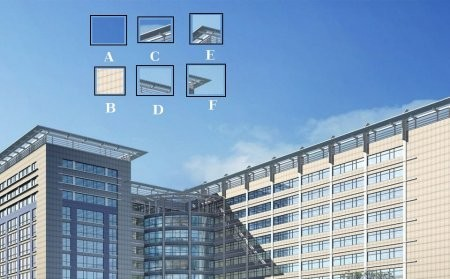
\includegraphics[width=0.7\textwidth]{features}
	\caption[Puntos de interés]{Eemplo de caracterizacion de pntos en una imagen}
	\label{imagen:features}
\end{figure}

Atendiendo a la imagen \ref{imagen:features}, se puede observar que se caracterizadas seis areas de interé. Analizando estos segmentos, vemos que \textbf{\textit{A}} y \textbf{\textit{B}} corresponden con superficies planas, lo que hace que sean muy dificil de identificas la ubicación exacta de esta superficie en la imagen completa. Por otro lado, tenemos las regiones \textbf{\textit{C}} y \textbf{\textit{D}}, las cuales corresponden con bordes en la imagen, si bien, se puede limitar en gran medida el area de busqueda pero de igual forma es dificil encontrar la ubicación exacta. Finalmente, analizando las regiones \textbf{\textit{E}} y \textbf{\textit{F}} tenemos que corresponden a esquinas de la imagen original, en este caso se puede identificar facilmente la ubicación exacta de la region en la imagen.

A partir de esta idea, en la cual se consideran las esquinas como regiones facilmente identificables en una imagen, en \textit{1988} nace el imprimer algoritmo de detección de puntos de interés \cite{harris} llamado Detector de esquinas de Harris.

Tomando la idea planteada previamente, este detector busca la diferencia de intensidad para cada desplazamiento de la ventada de busqueda, en todas las direcciones. Es decir se detectará una esquina, para aquellas regiones que presenten una alta variacion de intensidad al desplazar la ventana estudiada en todas las direcciones. En la figura \ref{imagen:harris-window} se puede apreciar visualmente como funciona esta ventana de busqueda.

\begin{figure}[H]
	\centering
	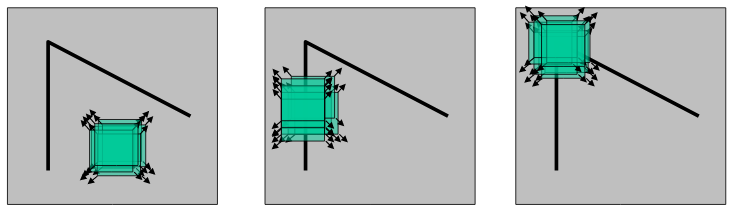
\includegraphics[width=0.9\textwidth]{harris-window}
	\caption[Deteccion de esquinas]{Desplazamiento de la ventana de busqueda, para de deteccion de esquinas}
	\label{imagen:harris-window}
\end{figure}

Cuando se trabajan con detectores de caracteristicas, se desea que estos sean invariantes ante la mayor cantidad de variables posibles, es decir, que sean capaces de detectar las mismas caracteristicas en una imagen a pesar de cambios en la traslación, rotación, escala, variaciones de iluminación, variaciones del punto de vista, entre otras. Si bien el detector presentado anteriormente es invariante ante la traslacion y la escala, ya que las esquinas se mantienen como esquinas si son rotadas o movidas, no funciona de la misma forma ante cambios de escala. Como se observa en \ref{imagen:corner-scale}, una región considerada como esquina, puede ser considerada plana si es ampliada.

\begin{figure}[H]
	\centering
	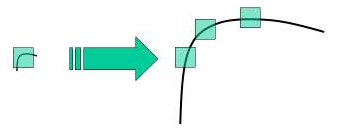
\includegraphics[width=0.85\textwidth]{corner-scale}
	\caption[Deteccion de esquinas]{Desplazamiento de la ventana de busqueda, para de deteccion de esquinas}
	\label{imagen:corner-scale}
\end{figure}

Otra caracteristica que se busca en estos algoritmos para lograr ubicar estos puntos claves en una imagen distinta, es la capacidad de describir estos puntos una vez se hayan detectado. Para esto los algoritmos descriptores, una vez tengan la ubicacion de los puntos caracteristicos se encargan de convertir la información de su alrededor en una serie de numeros, o un vector que permita diferenciar un punto clave de otro. Esta información tambien es necesaria que sea invariante ante las variablen antes mencionadas, para lograr una identificacion efficiente del mismo punto en distintas imagenes.

Partiendo de estos problemas, en \textit{2004} D.Lowe crea el detector \textit{SIFT} (del inglés: Scale Invariant Feature Transform), el cual presenta invarianza ante cambios en la escala. El proceso para la deteccion y descripcion de puntos de interes de este algoritmo, consta de cuatro pasos principales:

En primer lugar, realiza una deteccion de maximos en el espacio de la escala aplicando la diferencia gaussiana. Para esto, se aplica el filtro gaussiano con distintos tamaños de media (se tienen distintas escalas), luego restando estas imagenes para distintos pares de escalas se logra la diferencia de gaussianas. Posteriormente se buscan los maximos locales a lo largo del espacio (coordenadas X,Y) para cada correspondiente escala. Este proceso de deteccion se puede visualizar en  \ref{imagen:sift-escalas}.

\begin{figure}[H]
	\centering
	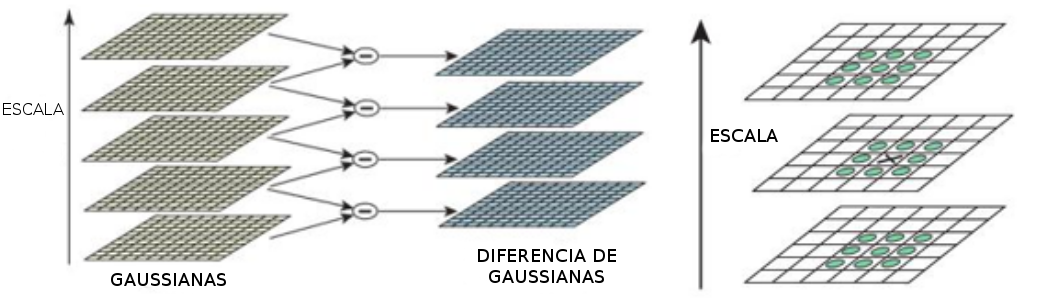
\includegraphics[width=0.85\textwidth]{sift-escalas}
	\caption[SIFT - Espacio de escalas]{Deteccion de maximos en el espacio de la escala}
	\label{imagen:sift-escalas}
\end{figure}

En segundo lugar para la localización de puntos de interés, se descartan los puntos encontrados en el paso anterior que no superen cierto valor de umbral, es decir, que no estén lo sufrientemente contrastados con su entorno. Con esta etapa el algoritmo solo toma en cuenta los puntos claves mas fuertes por cada escala. Además, con el objetivo de eliminar los bordes suficientemente contrastados que no correspondan con esquinas, el algoritmo usa una matriz hessiana para calcular las curvaturas principales, y así quedarse solo con esquinas.

Para garantizar la invariancia con respecto a la rotación, se toman los pixeles vecinos al punto clave y se calcula la magnitud y dirección del gradiente en esa región. Con esto se hace un histograma de la magnitud del gradiente en cada dirección, donde el pico mayor del histograma indica la orientación. En el caso que exista un pico mayor al 80\% del pico principal, este se utiliza para crear otro punto de interés en la misma posición pero con la distinta rotación.
Finalmente para la descripción por cada punto clave se crea una matriz de 16x16 alrededor de este, dividido en 4 subregiones de 4x4 pixeles con un histograma de orientaciones para cada uno. Finalmente, el descriptor del punto será el vector con los valores de los histogramas de las regiones 4x4 concatenados.

En el año 2006, David G. Lowe desarrolla un nuevo detector \cite{surf}, el cual está basado en SIFT, pero con modificacioes que cumentan su velocidad de detección. Si bien, sacrifica un poco de rendimiento y precision, lo hace mas provechoso para aplicaciones que demanden mayor velocidad de computo, como por ejemplo \textit{SLAM} (del ingles: Simultaneous Localization and Mapping). Las etapas para la extracccion se puntos se componen de la siguiente manera:

Como primer paso, en lugar de aproximar el laplaciano de Gauss (LoG) con la diferencia de Gaussianas (DoG) como lo hace SIFT, este algoritmo aproxima LoG con cuadrados para promediar la imagen. La ventaja de aplicar filtros con cuadrados es que con la ayuda de imágenes integrales el cálculo computacional se reduce en gran medida.

\begin{figure}[H]
	\centering
	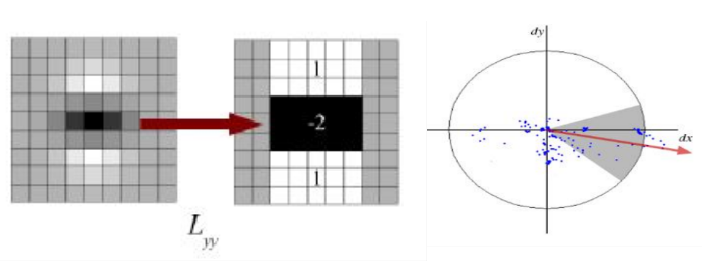
\includegraphics[width=0.8\textwidth]{surf}
	\caption[SURF - Espacio de escalas]{Deteccion de maximos en el espacio de la escala}
	\label{imagen:surf}
\end{figure}

En funcion de identificar la orientación, el algoritmo utiliza la respuesta wavelet Haar en horizontal y vertical en un vecindario de 6s (s es la escala del punto clave) pixeles al rededor del punto de interés, Luego estas respuestas son representadas como puntos en el espacio para luego calcular la orientación dominante con la suma de todos los resultados dentro de una ventana deslizante de apertura 60$^\circ$. En \ref{imagen:surf} se puede visualizar la forma del filtro que aplica el detector, y el vector de orientacion en funcion a la distribucion de puntos estudiados.

El siguiente avance importante en los algoritmos de deteccion aparece en el año 2001 con \textit{ORB} (del inglés: Oriented FAST and Rotated BRIEF) \cite{orb}, este utiliza una combinacion del detector FAST (del inglés: Features from Accelerated Segment Test) y del descriptor BRIEF (del inglés: Binary Robust Independent Elementary Features), caracterizado por su velocidad, gracias al uso de un descriptor binario y manteniendo un buen rendimiento. 

Como se mencionó utiliza el algoritmo FAST el cual consiste en encontrar esquinas evaluando los pixeles en un perimetro circular, de esta forma, un punto será detectado como si la cantidad de pixeles de color opuesto al evaluado supera cierto valor de umbral (ver izquierda en \ref{imagen:orb}), posteriormente con el fin de incrementar la cantidad de puntos, el algoritmo de esquinas de harris es aplicado. También se hace de forma piramidal evaluando varias escalas (al igual que SIFT).

Como el algritmo FAST no toma en cuenta la orientación, en el ORB se modificó para que calculara la orientación de la siguiente forma: se calcula a partir de la figura de una esquina (correspondiente al punto de interés) el centroide que le corresponde, luego se selecciona la orientación del vector que va desde este centroide hasta el centro de la esquina.

\begin{figure}[H]
	\centering
	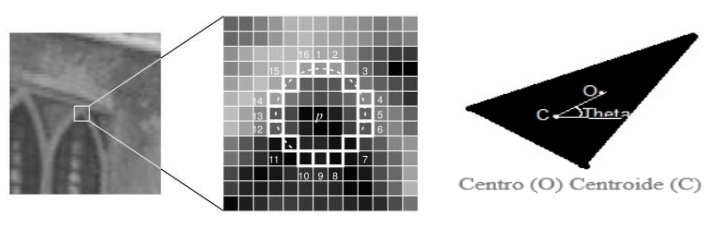
\includegraphics[width=0.9\textwidth]{orb}
	\caption[ORB - Espacio de escalas]{Deteccion de maximos en el espacio de la escala}
	\label{imagen:orb}
\end{figure}

Para el descriptor utiliza BRIEF, a diferencia de los anteriores (SIFT y SURF) este es un descriptor binario y no vectorial. El descriptor BFIEF produce una palabra de n-bits usando el algoritmo Local Binay Tests (LBT), el problema de esta representación es que no es muy robusta antecambios en la rotación. Para resolver esto ORB utiliza la información de la orientación previamente calculada para aplicar LBT en esa orientación y obtener la información del descriptor.

AKAZE: Detector y Descriptor
- Detector: Este algoritmo está basado en el descriptor KAZE, en cual tiene varias mejoras destinadas a aumentar la velocidad. A diferencia de los anteriores, el algoritmo AKAZE opera en espacios de escala no lineales, los algoritmos anteriores utilizan filtros gaussianos para detectar las características, mientras que AKAZE realiza una difusión no lineal en la imagen, lo que permite mantener ciertos detalles y eliminar ruido mientras se cambia de escala la imagen, a diferencia del filtro gaussiano que difumina los bordes y detalles de la imagen al cambiar de escala.

- Orientación: Este algoritmo utiliza un descriptor para la orientación similar al que emplea SURF, encuentra la orientación dominante en un área circular de radio 6s (s es la escala). Para cada muestra del círculo del descriptor se deriva en x e y, estos puntos se ubican en un espacio para calcular la orientación dominante en la orientación con más puntos.

\begin{figure}[H]
	\centering
	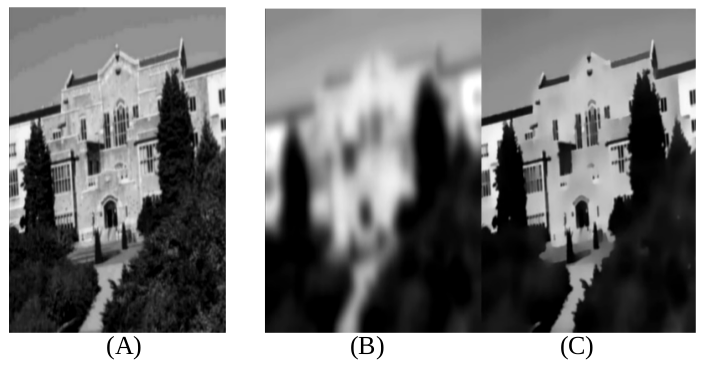
\includegraphics[width=0.85\textwidth]{kaze}
	\caption[KAZE - Espacio de escalas]{Deteccion de maximos en el espacio de la escala}
	\label{imagen:kaze}
\end{figure}

- Descriptor: Es descriptor de este algoritmo está basado en diferencia local binaria (LDB Local Difference Binary), el cual sigue el mismo principio que el BRIEF. Al añadirle una modificación para este algoritmo se le llamó M-LBD para que aproveche al máximo la información del espacio de escala no lineal. La modificación consiste en hacer un submuestreo de cada subregión que divide la zona del descriptor, en vez de sacar el promedio de todos los pixeles de la subdivisión, es decir, se tienen muestras de cada subdivisión para distintas escalas.


\section{Proyección de imagenes}


\section{Fusión de imagenes}

mensaje de prueba subsección 2

